\chapter{Assignment 5: Regularized Regression}


\section{problem statement}
Given data points $(x_i, y_i)$, $i = 1, \dots, n$, we aim to fit a polynomial model:
\begin{equation}
f(x) = \alpha_0 + \alpha_1 x + \alpha_2 x^2 + \dots + \alpha_{10} x^{10}
\end{equation}
where the parameters $\alpha = [\alpha_0, \alpha_1, \dots, \alpha_{10}]^\top$ are determined using Ordinary Least Squares (OLS) and ridge-regularized OLS.

\section{Procedure}
\subsection*{Step 1: Matrix Formulation}
we define

\begin{equation}
\mathbf{y} = 
\begin{bmatrix}
y_1 \\
y_2 \\
\vdots \\
y_n
\end{bmatrix}, \quad
\mathbf{X} = 
\begin{bmatrix}
1 & x_1 & x_1^2 & \cdots & x_1^{10} \\
1 & x_2 & x_2^2 & \cdots & x_2^{10} \\
\vdots & \vdots & \vdots & \ddots & \vdots \\
1 & x_n & x_n^2 & \cdots & x_n^{10}
\end{bmatrix}
\end{equation}
Then the polynomial model can be written as:
\begin{equation}
\mathbf{y} = \mathbf{X} \alpha + \epsilon
\end{equation}
where $\epsilon$ is the error term.

\subsection*{Step 2: OLS Estimate}
The OLS estimate minimizes the sum of squared residuals:
\begin{equation}
\hat{\alpha}_{OLS} = \arg \min_\alpha \|\mathbf{y} - \mathbf{X} \alpha\|_{2^{2}}
\end{equation}
The solution is given by:
\begin{equation}
\hat{\alpha}_{OLS} = (\mathbf{X}^\top \mathbf{X})^{-1} \mathbf{X}^\top \mathbf{y}
\end{equation}

\subsection*{Step 3: Ridge-Regularized OLS Estimate}
Ridge regularization adds a penalty term to control the magnitude of $\alpha$:
\begin{equation}
\hat{\alpha}_{Ridge} = \arg \min_\alpha \|\mathbf{y} - \mathbf{X} \alpha\|_2^2 + \lambda \|\alpha\|_2^2
\end{equation}
where $\lambda > 0$ is the regularization weight.

The closed-form solution is:
\begin{equation}
\hat{\alpha}_{Ridge} = (\mathbf{X}^\top \mathbf{X} + \lambda \mathbf{I})^{-1} \mathbf{X}^\top \mathbf{y}
\end{equation}
where $\mathbf{I}$ is the identity matrix.

\subsection*{Step 4: Computation}
\begin{enumerate}
    \item Construct $\mathbf{X}$ from the input data by calculating $x_i^k$ for $k = 0, \dots, 10$.
    \item Compute $\hat{\alpha}_{OLS}$ using the formula $(\mathbf{X}^\top \mathbf{X})^{-1} \mathbf{X}^\top \mathbf{y}$.
    \item Select a penalty weight $\lambda$. A common practice is to test multiple values ($ \lambda = 0.1, 1, 10, \dots $) and evaluate the solutions.
    \item Compute $\hat{\alpha}_{Ridge}$ using the formula $(\mathbf{X}^\top \mathbf{X} + \lambda \mathbf{I})^{-1} \mathbf{X}^\top \mathbf{y}$.
\end{enumerate}

\subsection*{Weight for the Penalties ($\lambda$)}
\begin{itemize}
    \item Ridge regression shrinks the coefficients, reducing the risk of overfitting. The choice of $\lambda$ is crucial: 
    \item Small $\lambda$: Minimal regularization, closer to OLS.
    \item Large $\lambda$: Higher regularization, biasing coefficients toward zero.
\end{itemize}

\subsection*{Results}

\subsubsection*{OLS Solution}

the OLS $beta$ estimates  are:

\begin{figure}
    \centering
    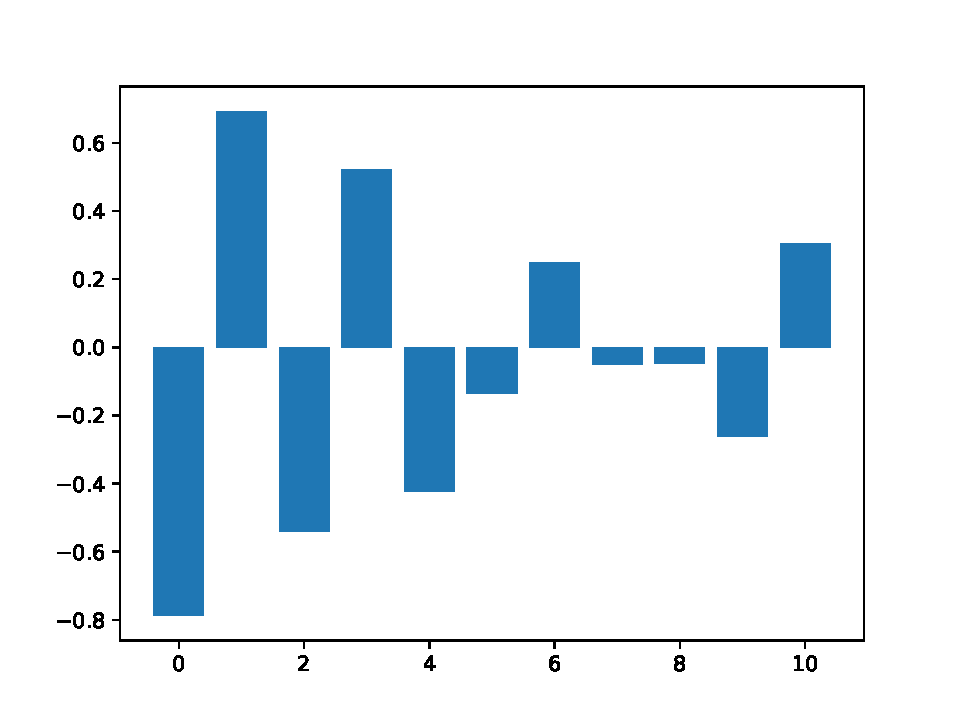
\includegraphics[width=0.8\textwidth]{figures/ols_beta.pdf}
    \caption{OLS $\beta$ Estimates}
\end{figure}

the OLS fits are shown in the following figure:

\begin{figure}
    \centering
    
\includegraphics[width=0.8\textwidth]{figures/ols_fit.pdf}
    \caption{OLS fits}
\end{figure}

\subsubsection*{Ridge Solutions}

There are few data, therefore the Ridge parameters were derived from a rmse search on all the data, without the train-test split.
The Ridge rmse with $\lambda = 0.5356$ is $1.8e+23$.
The fitted plot is shown below:
\begin{figure}
    \centering
    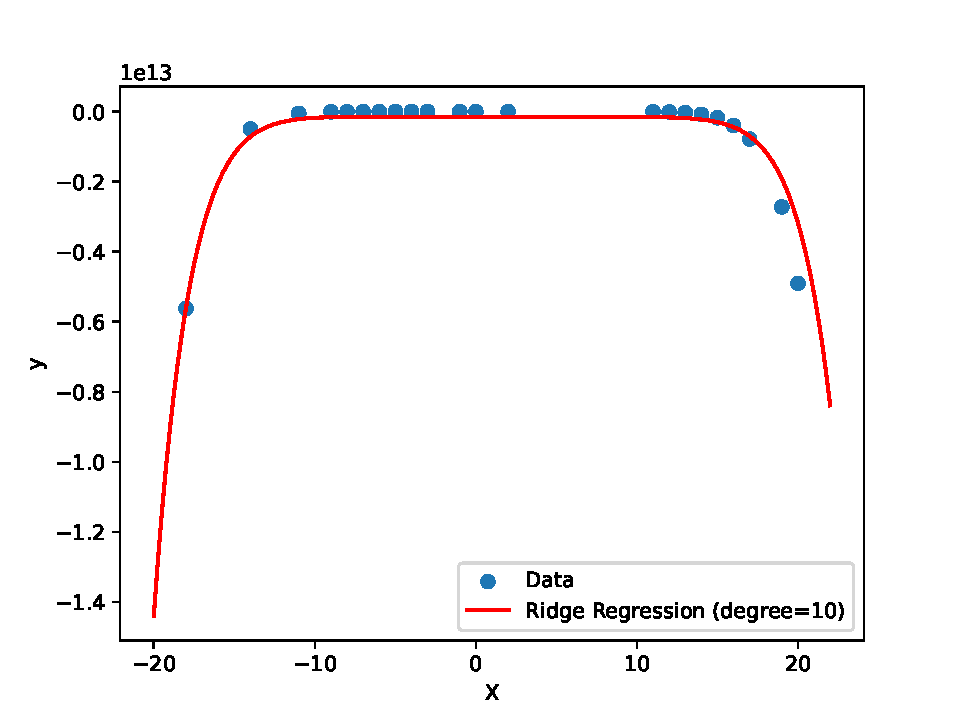
\includegraphics[width=0.8\textwidth]{figures/ridge_plot.pdf}
    \caption{Ridge fit}
\end{figure}



\subsection*{Qualities of Solutions}
\begin{itemize}
    \item OLS provides the best fit to the training data, but it may overfit if the model is too complex or if multicollinearity is present.
    \item Ridge regression balances the fit and model complexity, improving generalization by controlling the magnitude of $\alpha$.
\end{itemize}

\subsection*{Conclusion}
\begin{itemize}
    \item Use OLS for cases with low multicollinearity and sufficient training data.
    \item Use Ridge regression when multicollinearity exists or to reduce overfitting for high-degree polynomial models.
\end{itemize}

